\chapter{主体工作}

从上述整体设计出发,本研究的主要实现了SoCaffe — 一个基于深度学习框架Caffe并能运行于任一基于Zynq架构的嵌入式SoC设备上的深度学习框架。SoCaffe的名称来源于SoC与Caffe的结合。

本研究的主体工作可以分为如下三步:
\begin{enumerate}
\item 系统分析与架构设计:划分Caffe在SoC上的软硬件职责,确定CPU运行和FPGA加速的部分;
\item FPGA加速器实现:实现针对GEMM算法的硬件逻辑与应用优化策略;
\item ARM系统实现:构建数据通路、综合编译软硬件系统;
\end{enumerate}

本研究的最终成果包含编译好的基于FPGA的硬件加速库、使用硬件加速的Caffe链接库以及全部依赖的第三方链接库。使用本研究提供的Caffe版本与动态链接库,便可以直接实现基于Zynq SoC的深度学习应用。本研究的主体工作完全基于SDSoC工具实现:FPGA加速器使用了SDSoC包含的Vivado HLS工具进行硬件逻辑的编写与优化;数据通路构建依赖SDSoC提供的数据接口IP库;ARM系统的综合编译依赖SDSoC提供的ARM GNU编译工具链。

接下来按步骤介绍主体工作。

\section{系统分析与架构设计}

% Caffe的软硬件划分思路
只用ARM CPU完全足以运行Caffe,但性能不尽如人意。SoC上的CPU本身计算性能有限,而且难以并行化,因此需要FPGA硬件进行部分计算的硬件加速。由于GPU与FPGA在高性能计算的应用中拥有类似的特性,因此可以从Caffe的GPU加速函数中进行筛选,选择最适合FPGA计算的函数进行硬件加速。筛选的原则主要有以下三条:1)函数需要拥有较长的计算时间,占据总运行时间的很大比重,根据阿姆达尔定律(Amdahl's Law)加速类函数可以取得最大的加速比;2)代码逻辑简单,并行度高,适合在FPGA上运行;3)数据传输量小,不会花费很多时间在FPGA与CPU之间的数据传输上。从上述角度出发,本研究选用GEMM(GEneral Matrix Multiplicaion,通用矩阵乘法)作为在FPGA上主要优化的目标函数。

% 给GEMM简介
GEMM计算属于BLAS(Basic Linear Algebra Subprograms,基本线性代数子程序)集合,结合了矩阵乘法与加法计算:
\begin{equation}\label{eq:gemm}
\mathbf{C} \leftarrow \alpha op(\mathbf{A})op(\mathbf{B}) + \beta \mathbf{C}
\end{equation}

$\mathbf{A}$,$\mathbf{B}$,$\mathbf{C}$分别是输入矩阵,$\alpha$与$\beta$分别为GEMM计算的系数。此外,$op$函数会随着配置不同,对输入矩阵$\mathbf{A}$与$\mathbf{B}$不变换或者进行转置变换。因此GEMM具有充分的灵活性,可以配置出各种形式的矩阵乘法与加法组合。

% Caffe中对GEMM的使用
Caffe中大量使用了GEMM计算,主要在网络层的计算过程中,比如卷积层的卷积计算(\texttt{conv\_layer.cpp})。Caffe计算卷积的策略是把复杂的卷积操作变为简单的矩阵乘法问题,进而可以使用效率更高的、充分优化过的BLAS计算库。变换的方法主要是使用im2col操作对原始输入矩阵进行变换,把分离的矩阵块聚合起来\footnote{Caffe的作者贾扬清(Yangqing Jia)在这篇文章中解释了Caffe是如何使用GEMM与im2col来实现卷积层的:\url{https://github.com/Yangqing/caffe/wiki/Convolution-in-Caffe:-a-memo}}。总之,Caffe通过GEMM实现的卷积操作取得了不错的优化效果。

综上,整个深度学习框架在SoC上的划分如图3.1所示。处理系统上运行深度学习应用,并链接第三方链接库(比如OpenBLAS、LMDB等等)、caffe链接库(\texttt{libcaffe.so})与加速器链接库(\texttt{libaccel.so})。硬件加速器链接库提供调用FPGA硬件逻辑的高层接口。FPGA上主要实现了GEMM计算的硬件逻辑。PS与FPGA之间通过AXI总线和内存进行数据交互。
\begin{figure}[!ht]
\centering
	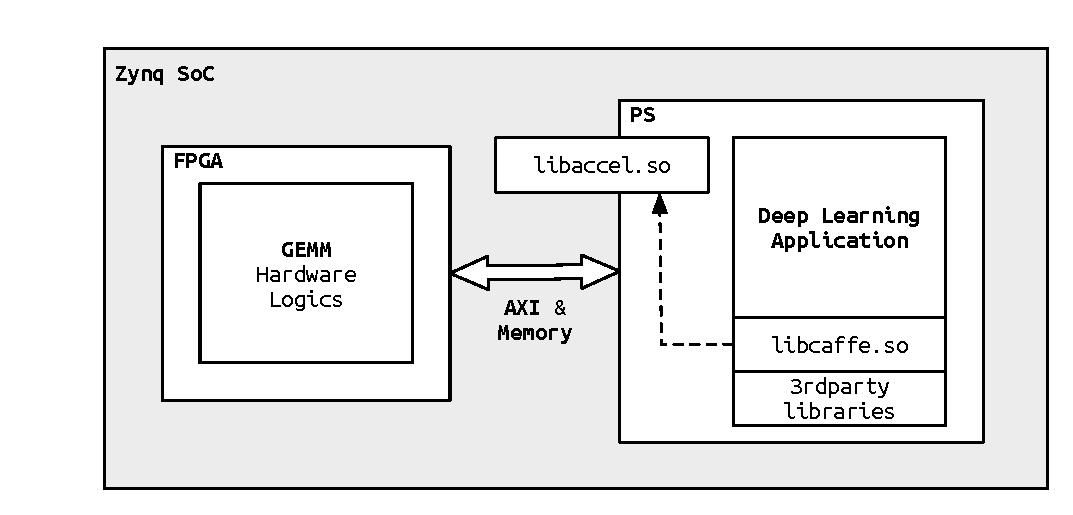
\includegraphics[width=0.9\textwidth]{assets/imgs/socaffe}
\caption{SoCaffe的系统架构}
\label{fig:socaffe}
\end{figure}

接下来分别介绍FPGA的加速器实现与ARM处理系统的实现工作。

\section{FPGA加速器实现}

基于FPGA实现的GEMM加速器是本研究的关键工作。本研究使用Vivado HLS工具设计并实现了基于固定大小的矩阵块之间的GEMM计算,并使用多种资源分配和调度策略进行优化;处理系统与FPGA之间的数据通路使用SDSoC工具提供的IP核实现;最后通过链接使得Caffe可以使用GEMM加速器进行计算。整个GEMM加速器基本使用了全部的FPGA硬件资源,相对于运行于CPU上的OpenBLAS库有5.45x倍速度提升,相应的测试结果在第四章详述。

\subsection{GEMM实现}

%% GEMM算法特性的介绍
GEMM本身并不复杂,以传统的三重循环实现的矩阵乘法为基础就可以在CPU上实现。下面的算法中以矩阵$\mathbf{C}$的行、列为优先,假设每次迭代的坐标为$(i,j)$。每次迭代首先把$\beta \times \mathbf{C}(i,j)$作为累积变量$sum$的初值,进而遍历矩阵$\mathbf{A}$和$\mathbf{B}$的$i$行与$j$列(如果$\mathbf{A}$或$\mathbf{B}$需要转置则使用$i$列或$j$行,算法的5、6行使用了C语言的三元条件表达式表示转置条件),将$\mathbf{A}$与$\mathbf{B}$的对应元素和$\alpha$相乘并累加。最后把$sum$赋给$\mathbf{C}(i,j)$。


\begin{algorithm}
\caption{GEMM的原始三重循环算法}
\label{alg1}
\algsetup{indent=2em}
\begin{algorithmic}[1]
\FOR{$i=0$ \TO $M$}
  \FOR{$j=0$ \TO $N$}
    \STATE{$sum \leftarrow \beta \times \mathtt{C[i][j]}$}
    \FOR{$k=0$ \TO $K$}
      \STATE{$a \leftarrow \mathtt{(TA)\ ?\ A[i][k]\ :\ A[k][i]}$}
      \STATE{$b \leftarrow \mathtt{(TB)\ ?\ B[k][j]\ :\ B[j][k]}$}
      \STATE{$sum \leftarrow \alpha \times a \times b$} 
    \ENDFOR
    \STATE{$\mathtt{C[i][j]} \leftarrow sum$}
  \ENDFOR
\ENDFOR
\end{algorithmic}
\end{algorithm}


\subsubsection{GEMM分块矩阵算法}
% 分块的原理
如果要将该算法移植到FPGA上,首先需要对矩阵计算进行分块。FPGA上只有有限的硬件资源,而且在计算开始之前已经固定,所以不可能进行使用该算法在FPGA上计算任意大小的矩阵。所谓分块(tiling),是指将原先以矩阵元素为单元的遍历方式,改变为以固定大小的矩阵块为单元的遍历方式。分块矩阵算法的基本原理是分块矩阵乘法与分块矩阵转置的计算公式(如图3.2,3.3)。

\begin{figure}[!ht]
\[
\begin{pmatrix}
  A_{1,1} & A_{1,2} & \cdots & A_{1,k} \\
  A_{2,1} & A_{2,2} & \cdots & A_{2,k} \\
  \vdots  & \vdots  & \ddots & \vdots  \\
  A_{m,1} & A_{m,2} & \cdots & A_{m,k} 
\end{pmatrix}
\times
\begin{pmatrix}
  B_{1,1} & B_{1,2} & \cdots & B_{1,n} \\
  B_{2,1} & B_{2,2} & \cdots & B_{2,n} \\
  \vdots  & \vdots  & \ddots & \vdots  \\
  B_{k,1} & B_{k,2} & \cdots & B_{k,n} 
\end{pmatrix}
=
\begin{pmatrix}
  C_{1,1} & C_{1,2} & \cdots & C_{1,n} \\
  C_{2,1} & C_{2,2} & \cdots & C_{2,n} \\
  \vdots  & \vdots  & \ddots & \vdots  \\
  C_{m,1} & C_{m,2} & \cdots & C_{m,n} 
\end{pmatrix}
\]

\caption{分块矩阵的乘法运算}
\end{figure}
\begin{figure}[!ht]
\[
\begin{pmatrix}
  A_{1,1} & A_{1,2} & \cdots & A_{1,k} \\
  A_{2,1} & A_{2,2} & \cdots & A_{2,k} \\
  \vdots  & \vdots  & \ddots & \vdots  \\
  A_{m,1} & A_{m,2} & \cdots & A_{m,k} 
\end{pmatrix}^T
=
\begin{pmatrix}
  A_{1,1}^T & A_{2,1}^T & \cdots & A_{m,1}^T \\
  A_{1,2}^T & A_{2,2}^T & \cdots & A_{m,2}^T \\
  \vdots    & \vdots    & \ddots & \vdots    \\
  A_{1,k}^T & A_{2,k}^T & \cdots & A_{m,k}^T 
\end{pmatrix}
\]

\caption{分块矩阵的转置运算}
\end{figure}

上述公式中的矩阵元素都是矩阵块,每个矩阵中的矩阵块大小一致。$m$,$n$,$k$分别为按照块大小划分后的矩阵中块的个数。分块矩阵乘法运算的结果中,每个结果矩阵块都是由块之间的乘法和累加构成的:
$$\mathbf{C}_{i,j}=\sum_{t=0}^{k} \mathbf{A}_{i,t} \times \mathbf{B}_{t,j}$$

而分块矩阵转置运算的结果相当于先以矩阵块为单元进行转置,之后分别对每个矩阵块进行内部转置。

从上述两个公式出发便可以得到GEMM的分块矩阵算法。$BLK\_M$,$BLK\_N$,$BLK\_K$分别为矩阵的块尺寸参数。本算法的框架基本与GEMM原始算法类似,但是其中计算参数都是矩阵块而不是矩阵元素。

\begin{algorithm}
\caption{GEMM的分块矩阵算法}
\begin{algorithmic}[1]
\FOR{$bi = 0$ \TO $\lceil M/BLK\_M \rceil$}
  \FOR{$bj = 0$ \TO $\lceil N/BLK\_N \rceil$}
    \STATE{$\mathbf{S} \leftarrow \beta \times \mathbf{C}_{bi,bj}$}   
    \FOR{$bk = 0$ \TO $\lceil K/BLK\_K \rceil$}
      \STATE{$\mathbf{A}_b \leftarrow \mathbf{A}_{bi,bk}$ or transposed $\mathbf{A}_{bk,bi}^T$}
      \STATE{$\mathbf{B}_b \leftarrow \mathbf{B}_{bk,bj}$ or transposed $\mathbf{B}_{bj,bk}^T$}
      \STATE{$\mathbf{S} \leftarrow \alpha \times \mathbf{A}_b \times \mathbf{B}_b + \mathbf{S}$}
    \ENDFOR
    \STATE{$\mathbf{C}_{bi,bj} \leftarrow \mathbf{S}$}
  \ENDFOR
\ENDFOR
\end{algorithmic}
\end{algorithm}


接下来具体介绍如何把分块矩阵算法实现于FPGA上。

\subsubsection{硬件加速实现}\label{subsubsec:normal}

FPGA上主要加速的是GEMM分块矩阵算法的第7行,对两个固定大小的矩阵块求乘法并进行累加。因此,矩阵块的大小不能任意取值,主要受限于FPGA的硬件资源数量:越大的矩阵需要越多的板上计算资源和存储资源。此外,为了适配Caffe的接口,该算法主要针对单精度浮点数格式设计实现。最后,为了简化FPGA实现的接口,CPU端会分配几个固定大小的矩阵块用来保存传输到硬件的参数。

\begin{figure}[!ht]
\centering
\includegraphics[width=\textwidth]{assets/imgs/gemm}
\caption{GEMM的软硬件设计}
\end{figure}

图3.4是具体的硬件加速设计架构:左侧为FPGA可编程逻辑,右侧为处理系统,二者之间通过AXI总线通信。如图所示,每次计算会先从矩阵中复制矩阵块到专门划分的缓存区中,如果有需要转置则在复制过程中进行转置(如算法2的第5,6行)。之后,FPGA把缓存的矩阵块放入BRAM中,在每个迭代步都进行矩阵乘法运算中的点积操作。矩阵$\mathbf{C}$也被读入,和点积结果进行累加。FPGA上的数据写回到矩阵$\mathbf{R}$中,防止与对$\mathbf{C}$的访问冲突。当计算完成之后,处理系统使用矩阵$\mathbf{R}$的结果对内存中的矩阵$\mathbf{C}$进行更新,每次更新一个矩阵块大小的数据。

上述GEMM加速系统的设计的软件端代码可以很容易地实现,但是硬件端代码主要有两部分组成:将总线中的数据复制到BRAM,以及从BRAM中读取数据进行计算。硬件逻辑代码如代码\ref{lst:gemmaccel}和代码\ref{lst:gemmaccelkern}所示。
\begin{listing}[!ht]
\inputminted[
  mathescape, 
  linenos,
  numbersep=5pt,
  breaklines=true,
  fontsize=\footnotesize]{c}{assets/codes/hls.c}

\caption{\texttt{gemm\_accel}函数的定义(未优化)}
\label{lst:gemmaccel}
\end{listing}

\begin{listing}[!ht]
\input{assets/codes/hlskern.tex}
\caption{\texttt{gemm\_accel\_kernel}函数的定义(未优化)}
\label{lst:gemmaccelkern}
\end{listing}

% 简单介绍代码的情况
这两份代码都默认矩阵块的大小必须完全相同,这是一种简化,在实际实现的代码中尺寸可以不一致(相应的论述参见第\ref{subsubsec:matshape}节)。\texttt{gemm\_accel}是被指定为要被HLS生成硬件的函数,因此\texttt{A\_buf},\texttt{B\_buf}与\texttt{C\_buf}都会被实现为FPGA上的BRAM\footnote{有的时候HLS工具也会用LUT来生成存储,选择BRAM还是LUT可以在程序中显式指定},\texttt{gemm\_accel}所调用的\texttt{gemm\_accel\_kernel}中的计算过程也会被实现为硬件逻辑。

\subsubsection{基本优化技巧}

两个函数中出现的循环一般会被实现为硬件逐步迭代进行的计算,但因为在代码中使用HLS的流水线预编译指令(pipeline),因此循环的迭代步之间可以同时执行:上一步迭代的计算与这一步迭代的BRAM读取不冲突,可以并行。流水线化是实现高效硬件逻辑的关键步骤,在Vivado HLS工具中,流水线化与循环控制流密切相关,被流水线化的循环内部的嵌套循环会被默认进行循环展开(Loop Unrolling)。同时,初始化间隔(Initialization Interval,简称II)指的是流水线需要几个时钟周期才能进行初始化,当II=1时流水线化达到最佳水平。II=1的结果主要因为对A和B的数组划分(Array partition):对A与B的访问可以同时通过多个端口进行,这样流水线便不会阻塞。

\subsubsection{数据通路}\label{subsubsec:interface}

数据通路主要由SDSoC生成,使用的是axis\_accelerator\_adapter这一AXI总线IP核\supercite{ug1027}。该IP核可以支持AXI4-Stream与AXI4-Lite两种模式,其中AXI4-Stream可以支持BRAM和FIFO接口。使用BRAM还是FIFO一方面可以由开发者通过预编译指令主动指定,另一方面也可以由SDSoC进行判断,如果内存块会被顺序访问的话,则使用FIFO,否则使用随机访问的BRAM。根据\ref{lst:gemmaccel}中对几个输入数组的访问模式,这些参数都是按照顺序进行访问的,因此可以使用预编译指令强行指定顺序访问。

\subsubsection{总结}
本节给出了基于分块矩阵算法的简单GEMM实现,其中用到了基本的流水线化、数组划分以及数据通路分析的技巧,而且也通过指定矩阵尺寸为32得到了性能和资源占用的报告。

但是存在两个问题:一是该实现的延迟过长(大于4000),最终得到的硬件效率不高;二是尺寸为32不一定是最好的结果,FPGA上还有很多空余资源可以使用。下一小节会对性能给出基本的分析和预测。


% 性能预测与高层次综合报告
\subsection{GEMM性能分析与预测}\label{subsec:predict}

% 前提假设
本节从GEMM算法的特性出发,找出性能与GEMM分块算法中的块大小之间的数学关系。性能指标的单位为GFLOPS(Giga floating-point operations per second,每秒1G次浮点运算操作个数)。由于GEMM分块算法有多种分块方式,为了简便起见本节中使用正方形划分的分块方式,即从矩阵$\mathbf{A}$,$\mathbf{B}$,$\mathbf{C}$划分出的任意块$\mathbf{A_{ik}}$,$\mathbf{B_{jk}}$与$\mathbf{C_{ij}}$都是正方形。此外,本节性能分析只涉及FPGA硬件逻辑的计算时间,数据传输延迟暂不考虑。

%% FPGA的性能预测概论
理论上,FPGA的运行时间($time_{HW}$)延迟($latency$,单位为时钟周期数)和时钟频率($freq$,单位为MHz)相关:

\begin{equation}\label{eq:timelatency}
time_{HW}=\frac{latency}{freq}
\end{equation}
% $$\mathtt{time} = \mathtt{latency} \times 1 / \mathtt{frequency} = 2352 / (143 \times 10^{6}) s = 1.64 s$$

% 延迟大小与GEMM块大小的关系
延迟的大小与GEMM使用的矩阵块大小密切相关。矩阵块大小由三个参数决定:$Dim_M$,$Dim_N$,$Dim_K$\footnote{$M$,$N$,$K$的语义与描述矩阵乘法的场景中使用的语义一致,即$Dim_M$为矩阵块$\mathbf{A_{ij}}$的高,$Dim_K$为其宽。其余可以类推得到。}。
原始实现(如\ref{subsubsec:normal}节所示)中延迟由两个子过程决定,分别为BRAM复制与GEMM计算。
%% BRAM复制与GEMM块大小的关系
BRAM复制过程包含三个独立的、流水线化的循环,总延迟(\(\mathit{L_{BRAM}}\))等于三个循环的延迟之和。
假设初始化间隔已经达到目标1,则流水线化的循环延迟约等于循环体的延迟\footnote{\(\mathbf{A}\)矩阵块的BRAM复制循环与其他循环不同,延迟主要取决于与\(\alpha\)的乘法计算延迟,因为乘法比赋值更慢}加上循环周期数,因此:
\begin{equation}\label{eq:bramcopylatency}
\begin{aligned}
\mathit{L_{BRAM}}
& = \mathit{L_{AMultLoop}+L_{BCopyLoop}+L_{CCopyLoop}} \\
& = \mathit{Dim_M\times Dim_K + L_{mult}} 
  + \mathit{Dim_N\times Dim_K + L_{copy}} \\
& + \mathit{Dim_M\times Dim_N + L_{copy}} \\
& = \mathit{S_A + S_B + S_C + 2L_{copy} + L_{mult}} 
\end{aligned}
\end{equation}
%对于固定大小矩阵块的GEMM计算而言,一次运算共进行$\mathtt{Dim}^3\times2+\mathtt{Dim}^2+\mathtt{Dim}^2\times 2 = 2\mathtt{Dim}^3+3\mathtt{Dim}^2$次浮点数运算。因此理论上GFLOPS(每秒G次浮点数运算)的结果为:
%$$\mathtt{GFLOPS} = (2\mathtt{Dim}^3+3\mathtt{Dim}^2)/\mathtt{time} = 4.17$$
即BRAM复制过程的延迟等于三个矩阵块的面积和与两个复制的延迟(\(\mathit{L_{copy}}\))、一个乘法运算的延迟(\(\mathit{L_{mult}}\))的和。
% 乘法计算与GEMM块大小的关系
GEMM计算延迟(\(\mathit{L_{comp}}\))取决于流水线化的GEMM三重循环计算,由于其中第二层循环被流水线化,这部分的总延迟等于前两层的循环周期数加上第三层循环完全展开后的点积计算延迟(\(\mathit{L_{prod}}\)):
\begin{equation}\label{eq:complatency}
\begin{aligned}
\mathit{L_{comp}}
& = \mathit{Dim_M \times Dim_N + L_{prod}} \\
& = \mathit{S_C + Dim_K \times L_{add} + L_{others}}
\end{aligned}
\end{equation}
简单对数据流进行分析可以发现,由于点积运算中包含存在依赖的求和运算,且这部分的延迟与\(\mathit{Dim_K}\)成正比
\footnote{根据\cite{ug902}第183页,对于浮点数格式的加法,为了防止出现精度问题,不会使用平衡过的加法树(Adder Tree),因此延迟与\(Dim_K\)的关系是线性而不是对数的。}
,因此GEMM计算延迟与\(\mathit{Dim_K}\)相关。

% 总延迟
综上,假定矩阵块面积的大小是主要决定因素(其他延迟变量的值暂且忽略不计),且令\(\mathit{Dim}\)为最大矩阵块尺寸,则综合公式\ref{eq:bramcopylatency}与\ref{eq:complatency},得到总延迟的表达式为:
\begin{equation}\label{eq:latency}
\begin{aligned}
\mathit{latency} 
& = \mathit{L_{BRAM}} + \mathit{L_{comp}} \\
& \approx \mathit{S_A + S_B + 2S_C} \leq 4Dim^2
\end{aligned}
\end{equation}
即总延迟的大小的上界为\(\mathit{4Dim^2}\)。

% 总浮点数操作数
GEMM的浮点数操作数总数(\(\mathit{FLOP}\))也取决与矩阵块尺寸。从GEMM的公式出发\ref{eq:gemm},得到(公式\ref{eq:flop}中的下标为特定的运算步,\(\mathit{Dim}\)依然为矩阵块尺寸中的最大值):
\begin{equation}\label{eq:flop}
\begin{aligned}
\mathit{FLOP} 
& = \mathit{FLOP_{\mathbf{AB}}} 
  + \mathit{FLOP_{\alpha\mathbf{AB}}}
  + \mathit{FLOP_{\beta\mathbf{C}}}
  + \mathit{FLOP_{\alpha\mathbf{AB}+\beta\mathbf{C}}} \\
& = \mathit{2 Dim_M\times Dim_N\times Dim_K + Dim_M \times Dim_N} \\
& + \mathit{Dim_M \times Dim_N + Dim_M \times Dim_K} \\
& = \mathit{2 S_C \times Dim_K + 3 S_C} \\
& \leq \mathit{2 Dim^3 + 3 Dim^2}
\end{aligned}
\end{equation}

%% GFLOP
综合公式\ref{eq:latency}与\ref{eq:flop}可得:
\begin{equation}\label{eq:gflops}
\begin{aligned}
\mathit{GFLOPS}
& = \mathit{\frac{FLOP}{latency} \times frequency \times 10^{-9}} \\
& = \mathit{\frac{2 Dim^3 + 3 Dim ^ 2}{4 Dim^2}\times frequency \times 10^{-9}} \\
& = \mathit{\frac{2 Dim + 3}{4} \times frequency \times 10^{-9}}
\end{aligned}
\end{equation}
随$\mathit{Dim}$的增加,$\mathit{GFLOPS}$上升。

% 结论
综上,GEMM计算的硬件性能与使用的矩阵块的最大尺寸成正比,因而优化的目标应为最大化GEMM中使用的矩阵块大小。矩阵块大小的上限取决于FPGA上各类资源的总量,和GEMM硬件设计使用各类资源的方式。接下来具体阐述如何通过修改HLS生成硬件设计的方式来优化GEMM的计算效率。

\subsection{GEMM硬件资源约束分析}\label{subsec:resanalysis}

本节给出各个FPGA资源的约束条件,通过求解一个线性规划模型来得到在给定FPGA资源个数情况下,能得到的最大GEMM矩阵块大小。由\ref{eq:gflops}可知,GEMM矩阵块越大性能越好,因此本节所得到的GEMM矩阵块大小也是对计算性能而言最优的。本节的FPGA资源约束条件是针对原始实现\ref{subsubsec:normal}分析得到的,其他约束条件在下一章(\ref{subsec:gemmopt})的优化技巧中给出。

必须指出的是,本节的资源约束条件在精度上有误差。首先,因为GEMM计算只是FPGA上硬件逻辑之一,还有数据通路和其他控制逻辑也占用FPGA的资源,所以本节求解的最大矩阵块尺寸可能最终无法实现;其次,HLS过程给出的硬件资源报告会略大于实际的实现结果,因为实际实现过程中会有资源共享等优化;再次,本节只求解了GEMM算法主要使用的FPGA资源(DSP,LUT,FFF和BRAM),对其他的资源占用暂不考虑;最后,本节只计算了主要占用资源的操作或变量,其他资源占用也没有计入。尽管如此,本节的结论基本上可给出GEMM矩阵块的理论上限,可以指导对矩阵块大小的设置。

\subsubsection{BRAM资源约束}
在高层次综合阶段,BRAM资源使用的都是BRAM18K,即一个BRAM有18Kb存储空间的配置。每个BRAM有两个端口,既可以配置为两个读端口,也可以配置为一个写端口、一个读端口。但是,BRAM18K的端口带宽是18bit,如果读取的数据宽度大于18bit则只能有一个读端口
% 有关SDP的脚注
\footnote{根据\cite{ds190}第16页对"Programmable Data Width"的描述,提到只有SDP模式才能对BRAM18K读取大于18b的数据。SDP即Simple Dual-Port,要求只能配置一个端口为读端口}。

% 给出板上缓存的占用
原始实现(\ref{subsubsec:normal})中,主要占用BRAM资源的是代码\ref{lst:gemmaccel}中的板上缓存:\texttt{A\_buf},\texttt{B\_buf}与\texttt{C\_buf},还有\texttt{R}。\texttt{R}也默认实现为BRAM,占用空间与\texttt{C\_buf}相同。
% 数组划分的问题
此外,为了能实现达到初始化间隔(II)为1的目标,必须对\texttt{A\_buf}与\texttt{B\_buf}均进行了数组划分,划分结果必须满足\texttt{A\_buf}的第二维、\texttt{B\_buf}的第一维能同时访问全部的数据。假定数据类型为单精度浮点数(\texttt{float}),则根据前面所述这里只能由一个读端口。因此,令获取数据类型字节数的函数为\texttt{sizeof()},并且假定数组划分后的每个子数组都能用一个BRAM18Kb装下
\footnote{本研究中没有使用到比BRAM18Kb限定的范围还要大的子数组,即没有矩阵块的任一维度大小大于576,所以这里假定暂时成立。}
,则可以得到\texttt{A\_buf}与\texttt{B\_buf}使用的BRAM数量(分别为\(\mathit{A_{BRAM}}\)和\(\mathit{B_{BRAM}}\)):
\begin{align}
\mathit{A_{BRAM} 
	= Dim_K \times 
	\lceil 
	\frac{Dim_M\times \texttt{sizeof(float)} \times 8}{18 \times 1024} 
	\rceil
	\approx Dim_K\lceil 1.7Dim_M \times 10^{-3} \rceil
	\approx Dim_K }
\label{eq:Abram}\\
\mathit{B_{BRAM}
	= Dim_K \times 
	\lceil 
	\frac{Dim_N\times \texttt{sizeof(float)} \times 8}{18 \times 1024} 
	\rceil
	\approx Dim_K\lceil 1.7Dim_N \times 10^{-3} \rceil
	\approx Dim_K}
\label{eq:Bbram}
\end{align}
即二者使用的BRAM其实与数组划分的对应维度大小,乘上由其他维度组成的数组所占用的BRAM个数相同。

%
% C的问题
\texttt{C\_buf}没有进行数据划分,因此可以直接按照其数据量大小进行计算,其使用BRAM18K的个数为:
\begin{equation}\label{eq:Cbram}
\begin{aligned}
\mathit{C_{BRAM} = R_{BRAM}}
& = \lceil \mathit{
	\frac{S_C\times \texttt{sizeof(float)} \times 8}
	{18 \times 1024\ bits}} \rceil
& \approx \lceil \mathit{1.7S_C \times 10^{-3}} \rceil
\end{aligned}
\end{equation}

% 给出IP核的占用
此外,尽管在代码中没有体现,但是SDSoC工具会为\texttt{gemm\_accel}函数生成处理输入与输出的IP核,如第\ref{subsubsec:interface}节所示。本节暂时不考虑这部分的BRAM使用。

% 总结
综上,假设FPGA上BRAM18K的资源为\(\mathit{Num_{BRAM}}\)个,则针对BRAM的约束条件为:
\begin{equation}\label{eq:bram}
\begin{aligned}
\mathit{A_{BRAM} + B_{BRAM} + C_{BRAM} + R_{BRAM}}
& = \mathit{2Dim} + \lceil \mathit{3.4 Dim^2 \times 10^{-3}} \rceil \\
& \leq \mathit{Num_{BRAM}}
\end{aligned}
\end{equation}

\subsubsection{计算资源约束}
本节只讨论针对DSP,FF和LUT的计算资源约束,其中DSP资源的类型为DSP48E。GEMM算法对计算资源的使用主要来自\ref{lst:gemmaccelkern}中第三层循环的点积计算。由于流水线化的目标是达到II为1,因此这里的乘法与加法必须满足延迟的要求。根据HLS的综合报告发现,针对这一部分的加法和乘法操作使用的资源如下表所示:

\begin{table}[!ht]
	\centering
	\begin{tabular}{|l|l|l|l|}
		\hline
			 & DSP48E & FF & LUT \\ \hline
		fadd & 2 & 324 & 424 \\ \hline
		fmul & 3 & 151 & 325 \\ \hline
	\end{tabular}
	
	\caption{单一加法操作(fadd)与乘法(fmul)操作使用的资源个数}
	\label{table:gemmres}
\end{table}

由于点积运算的次数为\(\mathit{Dim_K}\),因此针对运算资源的约束可以轻易得到:
\begin{align}
\mathit{Dim_K \times 2 + Dim_K \times 3} 
& = \mathit{5 Dim_K} \leq \mathit{Num_{DSP}} 
\label{eq:dsp} \\
\mathit{Dim_K \times 324 + Dim_K \times 151} 
& = \mathit{475 Dim_K} \leq \mathit{Num_{FF}} 
\label{eq:ff} \\
\mathit{Dim_K \times 424 + Dim_K \times 325} 
& = \mathit{749 Dim_K} \leq \mathit{Num_{LUT}} 
\label{eq:lut}
\end{align}

\subsubsection{求解最大矩阵块尺寸}\label{subsubsec:maxdim}
综合\ref{eq:bram}、\ref{eq:dsp}、\ref{eq:ff}、\ref{eq:lut}等约束条件,以及本研究使用的Zynq系列XC7Z020的资源限制\supercite{ds190}:

\begin{table}[!ht]
	\centering
	\begin{tabular}{|l|l|l|l|}
		\hline
		BRAM18K & DSP48E & FF & LUT \\ \hline
		140 & 220 & 106400 & 53200 \\ \hline
	\end{tabular}

	\caption{XC7Z0202的资源}
	\label{table:xc7z020res}
\end{table}

代入上述数值,可以得到\(Dim\)的四个上界:44(DSP48E),71(LUT),224(FF)。
并且将44代入BRAM约束条件\ref{eq:bram}发现满足约束。因此,原始实现主要受限于DSP的个数,最大能达到的矩阵尺寸上限为44。

综上,根据硬件资源约束条件和实际数据求解可以发现,原始实现没有很好地利用板上的全部资源,在达到最大矩阵尺寸时,只有LUT的资源占用为61.9\%,其它都小于40\%。下一节会利用本节的约束条件以及相关结论优化GEMM对资源的使用。

\subsection{GEMM优化}\label{subsec:gemmopt}

% 引言 介绍前文中提到的算法和设计的问题
本节首先解决第一小节提出的高延迟问题,通过合并几个复制循环即可实现。
之后主要解决上一节的硬件资源占用不均匀的问题,总体而言有如下几种解决方案:一种想法是将使用DSP资源的计算用LUT等资源实现。此外,通过牺牲精度、使用更小的数据类型来降低每个操作所占用的资源,进而提高矩阵块的大小也是一种关键优化策略。本节使用了固定小数点数据类型(fixed-point data type)进行优化。
此外,上节的约束条件只使用了最大矩阵块尺寸\(\mathit{Dim}\),尽管模型更清晰简单,但是实际上如果矩阵块形状不规则,那么在满足约束条件的前提下也可以得到更大的矩阵面积(GFLOPS与矩阵面积相关)。

\subsubsection{优化延迟}\label{subsubsec:latency}
在延迟的表达式\ref{eq:latency}中,三个复制循环占据了大量的时间(基本为3/4)。如果在编译代码的过程中对矩阵尺寸进行判断,强制$Dim_M=Dim_N=Dim_K$,则可以将三个复制循环合并为一个:
\begin{listing}[!ht]
	\inputminted[
  mathescape, 
  linenos,
  numbersep=5pt,
  breaklines=true,
  fontsize=\footnotesize]{c}{assets/codes/hlskern-copy.c}

	\caption{\texttt{gemm\_accel}函数:优化延迟}
	\label{lst:gemmcopy}
\end{listing}

修改式\ref{eq:bramcopylatency}可以得到BRAM复制步骤的延迟下降为$Dim ^ 2 + L_{mult}$,即只需要循环$Dim^2$次并且循环主体的延迟为最长的乘法计算。

但是上述要求三个尺寸都相等的条件过于严格了,不利于对硬件资源的分配优化。第\ref{subsubsec:matshape}小节给出一种令$Dim_K$的值不同的不规则矩阵计算方式,对本小节的过程给出了改进。

% 优化硬件资源分配
\subsubsection{优化硬件资源分配}\label{subsubsec:resalloc}

为了在不增加延迟的基础上降低DSP的使用,本研究将部分计算强制使用非DSP资源实现。默认的浮点数乘法与加法运算都需要同时占据DSP,FF与LUT来实现其功能(如表\ref{table:gemmres}),三者之间是有固定比例的,因此根据FPGA资源比例和计算使用的硬件资源比例可以确定DSP是决定矩阵尺寸上限的主要因素。

解决该问题的主要思路是改变默认的计算资源使用方式。通过使用Vivado HLS的resource预编译指令,就可以指定某个参数的计算一定要使用某一种资源来实现。一般情况下这种做法可以改善对DSP的依赖情况。但是,对于包含循环的设计而言,一个操作往往会在多次迭代中频繁使用。对于这种情况,如果将该运算完全用LUT或其他资源实现,可能会造成DSP的使用与LUT的使用再次失衡,甚至会导致LUT的使用超出系统上限。

综上,本研究提出一种有效地优化硬件资源分配,均衡不同资源使用的方法:通过手动指定使用DSP的操作的迭代范围,来最大化对硬件资源的利用(如代码\ref{lst:gemmaccelkernopt}所示)。

\begin{listing}[!ht]
\inputminted[
  mathescape, 
  linenos,
  numbersep=5pt,
  breaklines=true,
  fontsize=\footnotesize]{c}{assets/codes/hlskern-opt.c}

\caption{\texttt{gemm\_accel\_kernel}函数片段:优化硬件资源分配}
\label{lst:gemmaccelkernopt}
\end{listing}

上述代码有四个循环,分别为只使用综合资源、使用加法LUT实现、使用乘法LUT实现,都使用LUT实现四种情况。确定每个循环长度的具体数值依然可以用约束条件求解实现。在表\ref{table:gemmres}添加不使用DSP的运算单元得到:

\begin{table}[!ht]
	\centering
	\begin{tabular}{|l|l|l|l|}
		\hline
		& DSP48E & FF & LUT \\ \hline
		fadd 			& 2 & 324 & 424 \\ \hline
		fmul 			& 3 & 151 & 325 \\ \hline
		fadd\_no\_dsp 	& 0 & 374 & 556 \\ \hline
		fmul\_no\_dsp 	& 0 & 523 & 798 \\ \hline
	\end{tabular}

	\caption{添加无DSP占用的加法与乘法操作实现}
	\label{table:gemmresnodsp}
\end{table}

根据表\ref{table:gemmresnodsp},代入循环长度\(d_1,d_2,d_3,d_4\),得到四个约束条件如下:
\begin{align}
\mathit{5d_1+3d_2+2d_3} & \leq \mathit{Num_{DSP}} 
\label{eq:dspopt} \\
\mathit{475d_1+525d_2+847d_3+897d_4}& \leq \mathit{Num_{FF}} 
\label{eq:ffopt} \\
\mathit{749d_1+881d_2+1222d_3+1354d_4}& \leq \mathit{Num_{LUT}} 
\label{eq:lutopt]} \\
\mathit{d_1+d_2+d_3+d_4}& = \mathit{Dim_K}
\end{align}

求解上述模型,可以发现当\(\mathit{Dim_K}\)的值为56的时候上述约束条件是无解的\footnote{本研究使用WolframAlpha\url{(http://www.wolframalpha.com)}语言进行上述模型的求解,代码为:\\
\texttt{Reduce[\{}\\
\texttt{5x+3y+2z <= 220,}\\
\texttt{475x+525y+847z+897t <= 106400,} \\
\texttt{749x+881y+1222z+1354t <= 53200,} \\
\texttt{x+y+z+t = dimK,} \\
\texttt{x>= 0, y >= 0, z >= 0, t >= 0\}, \{x,y,z,t\}]};\\
\texttt{dimK}通过尝试的方法发现\(\mathtt{dimK \geq 58}\)时,程序给出无解提示。此外,LUT与FF资源可能被应用于别的应用逻辑,在实际求解的时候对两个资源的上界乘上0.9,降低可用资源上限。
	}。
考虑到不规则的数值有可能不利于矩阵块的划分,最后本研究使用\(\mathit{Dim_K}=56\)的情况作为该优化策略的最优矩阵块。同时,由于对所有矩阵尺寸有长度一致的假定,因此\(\mathit{Dim_M=Dim_N=56}\)。此时的资源占用为\footnote{HLS的资源占用报告中没有给出IP核与其他逻辑的资源占用,因此本表在最后一行也给出最终资源占用}:
\begin{table}[!ht]
	\centering
	\begin{tabular}{|l|l|l|l|l|}
		\hline
		资源类型 & BRAM18K  & DSP48E & FF & LUT \\ \hline
		HLS资源占用(\%) & 84 & 96 & 34 & 89 \\ \hline
		最终资源占用(\%) & 63.57 & 96.36 & 40.27 & 56.59 \\ \hline
	\end{tabular}
	
	\caption{最优化硬件资源分配}
	\label{table:gemmresopt}
\end{table}

上述资源占用中DSP资源与LUT资源基本均匀使用,但是BRAM和FF的占用还是相对较少,需要考虑其他的优化策略。有关该最优分配的性能参见第\ref{subsec:compare}章。

% 大小不等的矩阵块
\subsubsection{优化矩阵块形状}\label{subsubsec:matshape}
之前的假定是矩阵块的大小尺寸必须完全一致,主要是为了在数据复制的步骤中使用一套循环逻辑来降低延迟。但如果将条件放松一些,当$M$与$N$对应的块尺寸相等,$K$对应的块尺寸相异时,循环逻辑依然可以保持不变,只需要增加循环内部的条件判断即可。

允许大小不等的矩阵块的优点在可以更精细地调整硬件资源的使用。BRAM的使用由三个块尺寸同时决定,而计算单元只是由$Dim_K$此在DSP和LUT的资源达到上限的时候,还可以通过增加$Dim_M$与$Dim_N$来增大BRAM的资源占用,从而提高FPGA每次运算的运算量。

\begin{listing}[!ht]
\input{assets/codes/hlskern-irr.tex}
\caption{\texttt{gemm\_accel}函数:优化矩阵块形状}
\label{lst:gemmaccelopt}
\end{listing}

代码\ref{lst:gemmaccelopt}中\texttt{DIM}与\(\mathit{Dim_M}\)和\(\mathit{Dim_N}\)相等,\texttt{VEC}与\(\mathit{Dim_K}\)相等。修改约束\ref{eq:bram}为:
\begin{equation}
\begin{aligned}
\mathit{A_{BRAM} + B_{BRAM} + C_{BRAM} + R_{BRAM}}
& = \mathit{2VEC} + \lceil \mathit{3.4 DIM^2 \times 10^{-3}} \rceil \\
& \leq \mathit{Num_{BRAM}}
\end{aligned}
\end{equation}

由于\texttt{VEC}主要受限于第\ref{subsubsec:resalloc}小节的计算,值取为56。代入BRAM的个数140,并且预留5\%空间给其它逻辑,则\texttt{DIM}的上界可以求得为78
\footnote{即求解一个$2*56 + 3.4 \mathtt{DIM}^2 \times 10^{-3} \leq 140*0.95$不等式。}。但是最终实现的时候,如果\texttt{DIM}数值越大,则对时钟频率的要求会更高。在满足时钟要求的情况下,经过不断地尝试,这里能取到最大的\texttt{DIM}数值为64。最终的报告如下表:

\begin{table}[!ht]
	\centering
	\begin{tabular}{|l|l|l|l|l|}
		\hline
		资源类型 & BRAM18K  & DSP48E & FF & LUT \\ \hline
		HLS资源占用(\%) & 90 & 86 & 34 & 92 \\ \hline
		最终资源占用(\%) & 71.79 & 86.36 & 40.89 & 59.30 	\\ \hline
	\end{tabular}
	
	\caption{最优化矩阵尺寸}
	\label{table:gemmirropt}
\end{table}

% 使用half
\subsubsection{优化数据类型 — 半精度浮点数}\label{subsubsec:half}
尽管上述几种优化策略已经能在FPGA上部署很大的矩阵块,执行很快的GEMM算法了。但是针对某些特殊的场景,比如要求实时性的计算时,之前的优化结果尚并不如人意。在这些场合中,对速度的要求高过对精确度的要求,因此可以使用更低精度的数据类型来降低平均每次计算所用到的资源,进而增加板上部署的矩阵块的大小。

\begin{figure}[!ht]
\centering
\includegraphics[width=0.4\textwidth]{assets/imgs/half}
\caption{IEEE-754半精度浮点数的格式描述,图片来源\url{(https://en.wikipedia.org/wiki/File:IEEE_754r_Half_Floating_Point_Format.svg)}}
\label{fig:half}
\end{figure}

HLS提供了对IEEE-754标准\supercite{ieee2008754}中的半精度浮点数(Half-precision floating point)的支持,
其格式包含1个符号位,5个指数位和10个尾数位(图\ref{fig:half}),共16位。半精度浮点数已经广泛地应用于计算机图形学等领域了。这里的优化实现方法只是将板上BRAM存储的矩阵块都用半精度浮点数声明,不改变输入参数的类型与处理系统中声明的数据类型。在FPGA的计算内核中使用半精度浮点数进行强制类型转换。代码如下:

\begin{listing}[!ht]
	\input{assets/codes/hlskern-half.tex}
	\caption{\texttt{gemm\_accel}函数片段:优化数据类型}
	\label{lst:gemmaccelhalf}
\end{listing}

可以看出第3行对缓存的数据类型修改为\texttt{half},在内部进行复制操作的时候发生了强制类型转换。

当数据格式发生改变的时候,原先基于\texttt{float}假设设计的约束条件都需要进行修改:1)BRAM:由于此时单一数据只占用16个bit,则一个BRAM18K可以拥有两个读端口,并且\texttt{C\_buf}占用的数据空间也需要修改,而由于\texttt{R}依然使用浮点类型,其数据占用不变。2)计算资源:此时使用的计算单元为\texttt{hadd}与\texttt{hmul},基本不使用DSP资源。

经过测试,使用半精度浮点数的GEMM算法可以使用最高达到$Dim=96$\footnote{此时依然可以使用不规则矩阵块的优化,但是如果把\(\mathit{Dim_K}\)增到很大,则会造成传输的数据量过大,不能满足时钟频率的情况}的矩阵块。
	
\begin{table}[!ht]
	\centering
	\begin{tabular}{|l|l|l|l|l|}
		\hline
		资源类型 & BRAM18K  & DSP48E & FF & LUT \\ \hline
		HLS资源占用(\%) & 80 & 43 & 30 & 40 \\ \hline
		最终资源占用(\%) & 92.50 & 43.64 & 38.51 & 52.17 	\\ \hline
	\end{tabular}
	
	\caption{修改数据类型的综合报告}
	\label{table:gemmhalf}
\end{table}
	
综上,GEMM的优化目标是尽可能地利用FPGA的资源,以部署更大的矩阵块来提高计算效率。使用了这一系列优化方式之后,GEMM自身相对于纯CPU的实现已经取得了很大的加速比。下一节具体描述如何令Caffe运行于Zynq SoC上,并与GEMM加速器相结合。

\section{ARM系统实现}

SoCaffe在处理系统上的工作(如图\ref{fig:socaffe})主要分为三个部分:编译与优化使用硬件加速库、交叉编译Caffe与其他第三方库、生成SD卡文件包。本节的工作主要依赖SDSoC工具,使用其提供的IP核、代码生成来构建与FPGA加速器的通信机制,ARM GNU工具链构建动态链接库和交叉编译,bootgen等工具生成包含比特流的Linux系统镜像等等。

% 链接加速器库
\subsection{构建与使用硬件加速库}

尽管在Caffe中使用GEMM加速库只用调用封装好的硬件加速器入口函数即可,但还有些问题需要考虑。首先,GEMM加速器并不适合全部形状的矩阵参数:当矩阵尺寸比较小时,使用GEMM加速器甚至比软件版本慢很多,主要原因是GEMM加速器的额外开销与计算对小尺寸矩阵计算时间而言是显著的。其次,在执行GEMM硬件加速函数的同时,CPU也应该利用起来,进行一些内存分配和复制等等简单操作,这就要求对GEMM硬件函数的调用代码需要异步执行。最后,GEMM硬件加速库与一般软件库不同,其中包含了一个硬件的比特流,选择何时加载、如何加载比特流也是需要考虑的问题。接下来会逐一讨论如何构建与使用GEMM硬件加速库。

\subsubsection{PS-PL接口生成}
调用GEMM加速器函数时,会以处理系统分配好的内存地址作为参数,SDSoC主要根据参数对应的内存块的分配方式来确定生成什么样的接口。如果内存块是以\texttt{malloc}分配生成的,则SDSoC使用Scatter-Gatter类型的接口访问内存中的数据。如果内存块以\texttt{sds\_alloc}分配,则SDSoC可以认识到该内存块是地址连续的,因此会使用顺序访问的接口(比如AXIDMA\_SIMPLE)。除此以外,如果不需要保证缓存的数据一致性,可以指定SDSoC生成使用AFI端口的高速访问数据通路,否则SDSoC会自动使用ACP端口。

\subsubsection{调用方式与条件}

% TODO 之后实现
% 在进行GEMM计算的同时,CPU端往往处于空闲状态。如果此时可以进行一些比较耗时的操作,比如复制数据到矩阵块缓冲区等等,那么系统性能可以得到不错的提升。SDSoC提供了预编译指令\texttt{async <ID>},用来标识硬件函数需要被异步调用;同时也提供了\texttt{wait <ID>}指令来指定等待硬件函数完成的时间点;其中\texttt{<ID>}用来对异步调用任务进行标记。这种异步机制本质上而言构建了FPGA与CPU之间的流水线,提高了系统的并行度。

正如本节序言所述,GEMM加速器是针对固定大小的矩阵块实现的,因此无法根据输入矩阵的形状进行调整。尤其是当输入矩阵形状非常不规律时,比如一条边很短($\sim 10$)而另一些边很长($\geq 1000$)时,使用GEMM加速器会带来非常大的性能损耗。本研究使用一种简单条件来判断是否应该执行GEMM:只有当输入矩阵的三个尺寸都大于128\footnote{128的数值主要根据第4章中对OpenBLAS的对比测试得到,当矩阵尺寸大于128时,GEMM加速器相对于OpenBLAS的性能才有了明显提升}时才调用GEMM加速器(如代码\ref{lst:caffegemm}所示,其中当定义了\texttt{SDS}时才会编译\texttt{gemm\_sds}接口),否则使用CPU端的BLAS库。

\begin{listing}[!ht]
\input{assets/codes/caffegemm.tex}
\caption{\texttt{caffe\_cpu\_gemm}函数}
\label{lst:caffegemm}
\end{listing}

代码中的\texttt{gemm\_sds}接口是对算法\ref{alg:gemmblocking}的直接实现,参数列表与\texttt{cblas\_sgemm}的标准一致,这里不加赘述。

\subsubsection{链接库生成}

传统的Zynq SoC应用开发在完成硬件函数的设计之后,是无法使用类似于软件方式调用该硬件逻辑的:必须要通过配置AXI总线的数据并传输数据才能执行硬件逻辑。但使用SDSoC进行开发时却可以直接调用硬件函数,究其原因,主要是因为SDSoC在编译过程中对原始的硬件函数进行了封装,并将封装后的版本替换了原始的函数调用。封装的函数包含了额外的数据准备,信号传输与等待命令完成等一系列过程。正因为如此,SDSoC可以为FPGA硬件逻辑自动构造出一个软件动态链接库。

但硬件逻辑的比特流却不包含在动态链接库中,而是放在一个独立的数据文件中。比特流文件可以在系统引导的过程中加载,也可以在系统运行过程使用\texttt{xdevcfg}设备动态配置。

% 交叉编译
\subsection{交叉编译}

所谓交叉编译,指的是一种编译出来的程序是运行在其他环境中的编译过程。SDSoC中提供的ARM GNU工具链就是在x86环境中交叉编译出ARM环境中可执行代码的交叉编译工具。使用该工具链编译GEMM硬件加速库,以及Caffe本身都很简便,但是涉及到Caffe的第三方库依赖便会遇到很多问题。针对第三方库的交叉编译主要有三种策略:

\begin{enumerate}
\item 直接修改环境变量中的\texttt{CC},\texttt{LD}等为ARM GNU工具链中对应的工具,可以用来处理比较简单的库的编译;
\item 使用第三方库提供的配置方案进行交叉编译配置:大部分第三方库都会使用configure、CMake等工具生成\texttt{Makefile},以方便交叉编译; OpenBLAS在编译工具链的配置之外也会要求指定对应系统架构的名称,进而可以充分优化性能\footnote{根据OpenBLAS的文档\url{(https://github.com/xianyi/OpenBLAS/blob/develop/README.md)},Zynq-7000搭载的Cortex-A9 ARM CPU应该使用\texttt{ARMV7}模式配置,该配置可以使用处理器上的浮点数计算硬件。但是由于SDSoC中附带的ARM GCC是Lite版本,不支持编译使用硬件浮点数计算单元,因此本研究中编译OpenBLAS为\texttt{ARMV5}模式,即所有运算都是软件实现的,没有使用浮点数处理器加速。}。
\item 其他:有的第三方库完全不支持交叉编译,主要原因是编译过程需要得到编译结果测试的反馈。比如HDF5在编译的过程中,会调用编译出来的程序来生成与目标系统相关的代码,处理起来非常麻烦\footnote{HDF5的官方文档明确指出不支持交叉编译\url{(https://www.hdfgroup.org/HDF5/faq/compile.html)},但根据邮件列表中的一封指南\url{(https://lists.hdfgroup.org/pipermail/hdf-forum_lists.hdfgroup.org/2013-September/007104.html)},经过一些复杂的CMake设置是可以完成编译的。本研究就是采用上述方法最终完成HDF5的交叉编译。}。
\end{enumerate}

因为第三方库的交叉编译标准不一,而且目标环境相对固定,因此本研究提供一套已经编译好的第三方动态链接库供SoCaffe使用,不需要重复编译,直接链接即可运行。

% 其他细节
\subsection{系统生成}

系统生成过程需要得到最终的、可用的SoCaffe系统,其中要包含编译好的动态链接库,FPGA比特流,以及其他工具等等。本研究按照如下流程构建SoCaffe系统:

\begin{enumerate}
\item 编译硬件加速器动态链接库(\texttt{libaccel.so}),生成包含FPGA比特流的SD卡与相应的引导文件;
\item 编译Caffe链接库(\texttt{libcaffe.so}),并链接第三方库函数和硬件加速器函数;
\item 编译使用SoCaffe环境的代码,比如各种基于Caffe的深度学习应用等等;
\item 将所有生成的链接库,可执行程序复制到第一步生成的SD卡目录中,进而复制到Zynq SoC使用的SD卡;
\item 启动系统,将链接库复制到系统库目录下(\texttt{/lib}),运行需要执行的程序;
\end{enumerate}

\section{总结}

本章首先给出了系统架构划分的思路,根据Caffe的软件架构和计算特性,决定只把GEMM操作移植到可编程逻辑中,其余功能在处理系统中实现。GEMM在FPGA上的移植分为三步,首先对传统软件算法进行改进,实现对FPGA优化的分块矩阵算法;然后对原始实现版本进行性能分析与预测,并给出优化的方向—修改硬件资源的占用方式;最后实现了各种不同的优化策略。此外,也需要对Caffe中对GEMM算法的调用进行修改,编译第三方链接库,并完成整个系统的生成。

下一章对SoCaffe进行完整详细的测试。